\documentclass[11pt]{article}
%Gummi|065|=)
\title{\textbf{Homework 5}}
\author{Anastasiia Khaburska}
\date{}
\usepackage{graphicx}
\usepackage{listings}
\graphicspath{ {./} }
\begin{document}

\maketitle

\section{Paper review}

 \textbf{Paper}
   \begin{itemize}
     \item \textbf{Title}: Good News, Everyone! Context driven entity-aware captioning for news images
     \item \textbf{Authors}: Ali Furkan Biten, Lluis Gomez, Marçal Rusiñol, Dimosthenis Karatzas
     \item \textbf{Link}: https://arxiv.org/abs/1904.01475
     \item \textbf{Tags}: Neural Network, image captioning, GoodNews dataset, context driven, entity-aware, attention algorithm
     \item \textbf{Year}: 2019
     \item \textbf{Code}: https://github.com/furkanbiten/GoodNews 
    \end{itemize}
\textbf{Summary}
     \begin{itemize}
     	\item \textbf{What}:
       \begin{enumerate}
			\item Latest state-of-the-art models for image captioning extract visual information by deep CNNs and then natural language descriptions are generated with RNNs. Despite the good results, simple sentences generally limited on enumerating or describing visual contents, and not offering any deeper semantic interpretation. Also, there exists a problem of dealing with named entities
			\item In this article, authors represent novel captioning pipeline, able to leverage contextual information to produce image captions at the scene interpretation level.
			\item A two-stage, end-to-end architecture, that allows to dynamically extend the output dictionary to out-of-vocabulary named entities that appear in the context source and are only made available at test time.
			\item Authors collected GoodNews -- the largest news image captioning dataset in the literature, comprising 466,000 image-caption pairs, along with metadata. 
       \end{enumerate}
        \item \textbf{How}:
       \begin{itemize}
			\item  Authors used the New York Times API to retrieve the URLs of news articles ranging from 2010 to 2018. 466, 0000 images with captions and text articles where randomly splitted into 424, 000 for training, 18, 000 for validation and 23, 000 for testing. 
			\item Model consists of two consecutive stages:
			\begin{enumerate} 
				\item Template caption generation
					\begin{itemize}
						\item Given an image and the text of the corresponding news article, a template caption is generated. The placeholders are introduced to indicate the positions of named entities and their respective tags.
						\item In general a word is produced at each timestep given the previously produced word and the attended image features, trained with cross entropy.
						\item More formally:
        	
        	$$s_i := {w_0, w_1, ..., w_N}$$, where $w_i$ is a vector for the $i$th word.       	
        	$$x_t = W_e*w_t, where\ t\in\{0,1,...,N-1\}$$        	
        	$$o_t = LSTM(concat(x_t, I_t, A_t))$$      	
        	$$w_{t+1} = softmax(W_{ie}o_t$$        	
        	$$L=-\sum_{t=0}^{N}{log(w_{t+1}})$$, where $W_e, W_{ie}$ are learnable parameters. $A_t$ denotes attended article features, and $I_t$ the attended image features.

The attended image features at timestep $t$ are obtained as a function of the hidden state of previous timestep and the image features extracted using a 5-th layer of $ResNet$ CNN model pretrained on $ImageNet$
			$$I_f = ResNet_5(I)$$
			$$I_t = Att(h_{t-1}, I_f)$$
, where I is the input image.
		
		Sentence level encoding can take into account the domain, purpose and context. It calculates the article's sentence level features $A_f \in R^{M*D_w}$, where $M$ - number of  sentences in the article and $D_w$ - length of the word vector obtained from the pretrained GloVe model. 
		
		Three methods of computing sentence level features where considered: Simple average, Weighted average and tough-to-beat baseline(TBB), which consists in subtracting the first component of the PCA from the weighted average of the article encoding since empirically the top singular vectors of the datasets seem to roughly correspond to the syntactic information or common words 

        			\end{itemize}
      			\item  Named Entity Insertion
      			
      			Selects the right named entities to fill placeholders with the help of an attention mechanism over the text of the news article.
      			
      			The attention mechanism works by multiplying the sentence level features with an attention vector $\beta_t \in R^M$ : $A_t=\beta_t*A_f$.
      			
      			The attention vector is learned with a fully connected layer, given the previous timestamp of the LSTM $h_{t-1}$ and the article features. $\theta_t=FC(h_{t-1}, A_f)$; $\beta_t=softmax(\theta_t)$
      			
      			Named entities in both captions and articles are recognized by the SpaCy’s named entity recognizer
			\end{enumerate} 		
       \end{itemize}
       	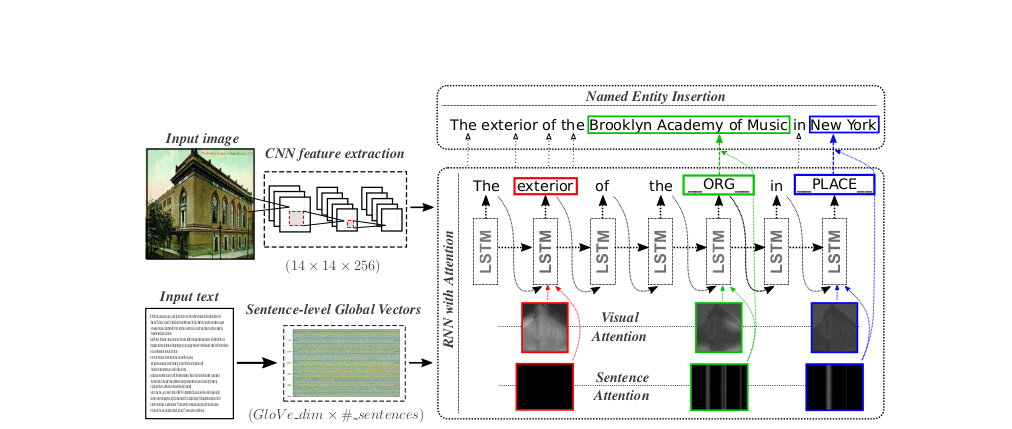
\includegraphics[width=\textwidth, height=7cm]{model}	
       	\item \textbf{Results}
       	
       	\begin{itemize}
			\item Experimental results demonstrate that the proposed method yields state-of-the-art performance on the intermediate task of \textbf{template caption generation}.
			\item It satisfactorily \textbf{incorporates named entity} information in the produced captions.
			\item Also, the adventages of \textbf{the Attention Insertion algorithm}, compared to Context-based Insertion, which computes the cosine similarity between sentence of the article and the template caption, are shown.
			\item The \textbf{human evaluation comparative study} revealed that the proposed model in \textbf{53\% } of cases was perceived better  than Show Attend and Tell + CtxIns model, which outperforms the rest of the baselines on the intermediate task of template caption generation. Also, the results indicate a consistent preference for the "visual+textual" than "just visual" variant.
		\end{itemize}
     \end{itemize}
     
\section{CNN visualization}
The features of the input image are extracted from the 5th layer of ResNet-152 network pretrained on ImageNet.

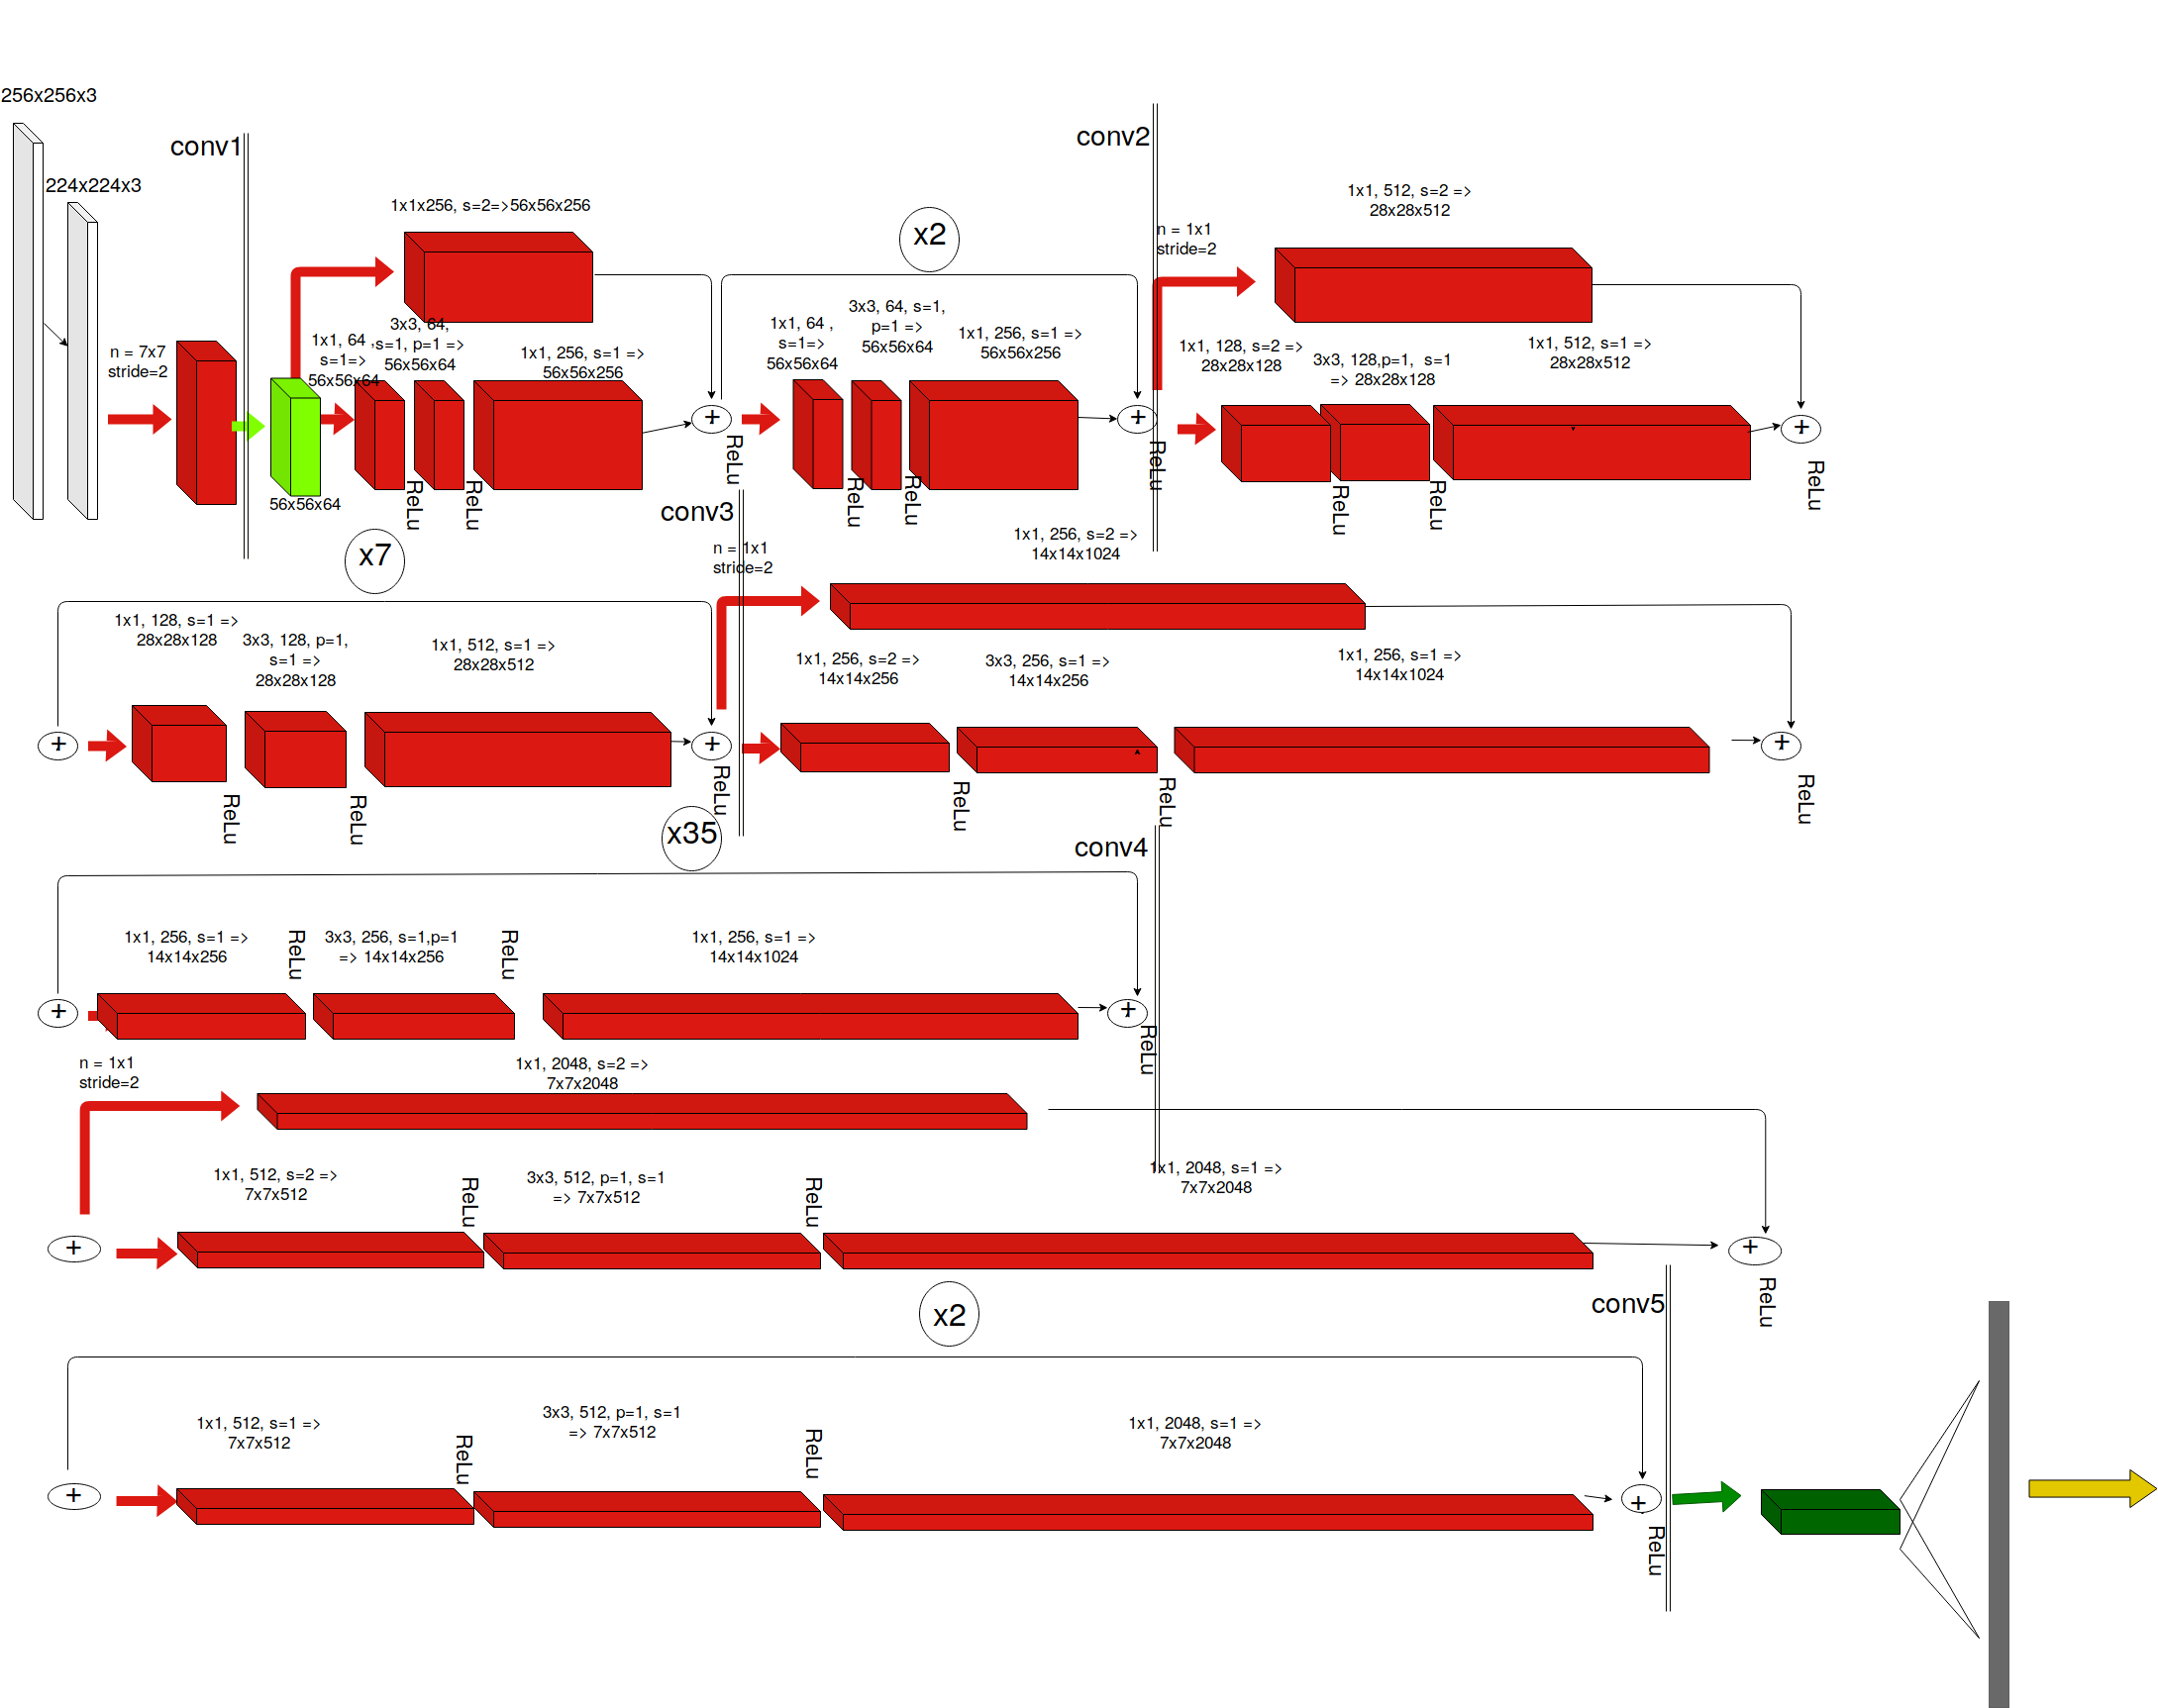
\includegraphics[width=\textwidth, height=12cm]{resnet}	

\section{Experiment summary}

1) 
	Task:
	\begin{itemize}
    \item create separate plots with 'epoch vs. loss' (in addition to the current 'iteration vs. loss')
    \item create separate plots with 'epoch vs. accuracy(train)'
    \item create separate plots with 'epoch vs. accuracy(test)' (for this create separate tag 'Test')
     \end{itemize}
     Solution:
     
     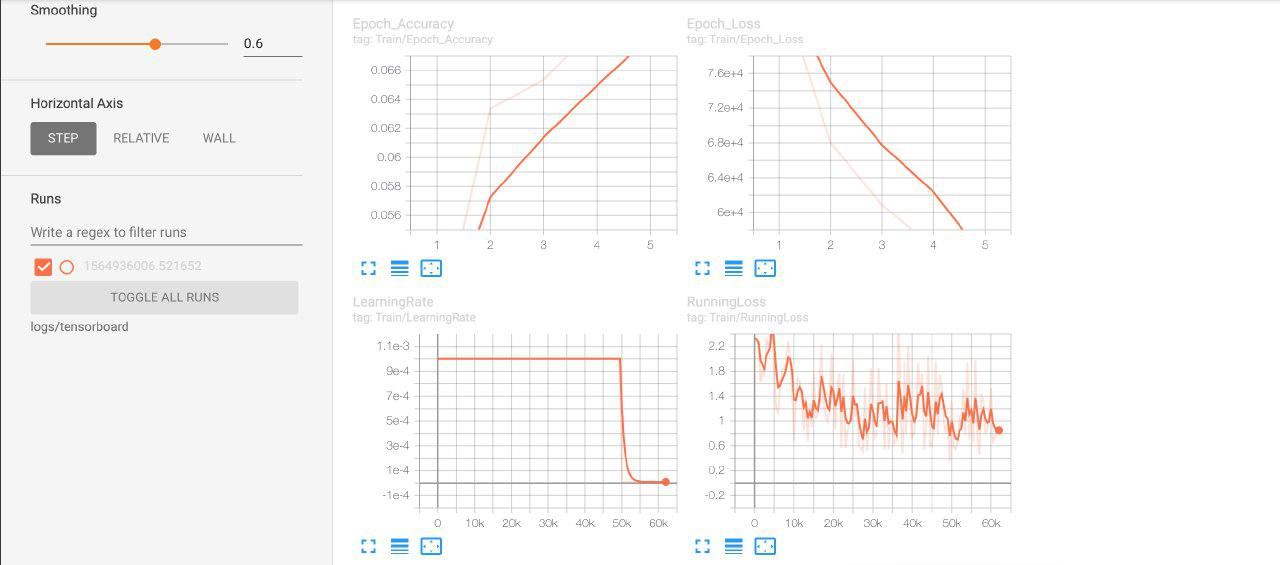
\includegraphics[width=\textwidth, height=7cm]{acurtrain}	
      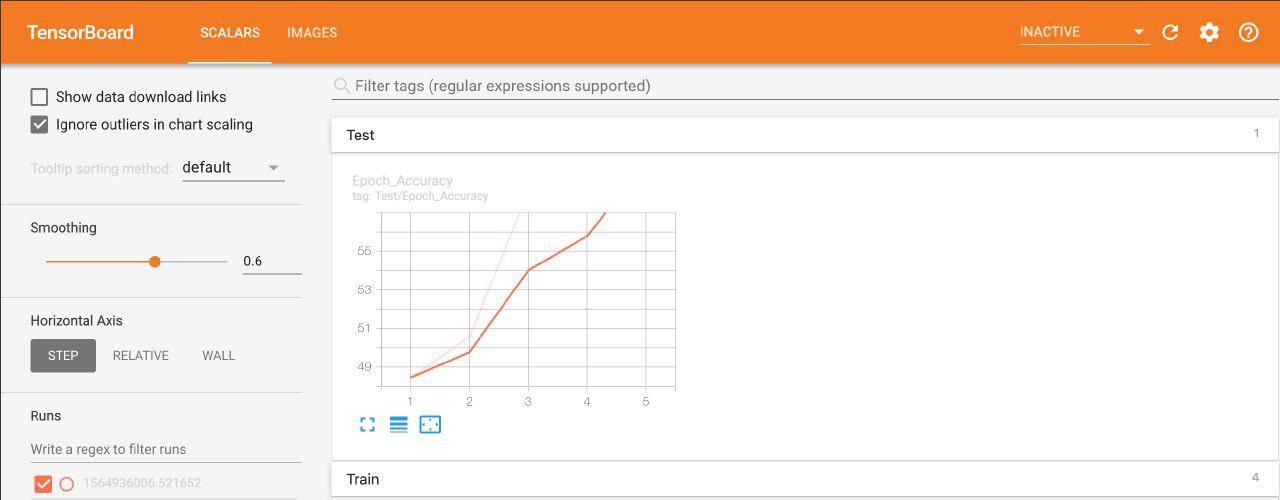
\includegraphics[width=\textwidth, height=7cm]{acurtest}
     
2) Augmentation

I used standart for CIFAR10 RandomCrop,RandomHorizontalFlip and of course Normalization. For test - only normalization.

\begin{lstlisting}
import torchvision.transforms as transforms
transform_train = transforms.Compose([
    transforms.RandomCrop(32, padding=4),
    transforms.RandomHorizontalFlip(),
    transforms.ToTensor(),
    transforms.Normalize((0.4914, 0.4822, 0.4465), (0.2023, 0.1994, 0.2010)),
])

transform_test = transforms.Compose([
    transforms.ToTensor(),
    transforms.Normalize((0.4914, 0.4822, 0.4465), (0.2023, 0.1994, 0.2010)),
])
\end{lstlisting}

3) Batch size : better results where shown by increasing batch size to 10

4) Optimizer: I tried different, but the best results where shown by Adam optimizer, so all the graphics in my report are with this optimizer 

5) Batch normalization:
Simply adding batch normalization, batchsize = 10, optmizer = Adam to the Net() class increased the accuracy on test set to 67%

6) GPU
This took me lots of time, but I managed to train neural networks on gpu. of course the speed is impressive

7) Out of simple CNNs that I trained, the best results where shown by the one from this tutorial: 
https://zhenye-na.github.io/2018/09/28/pytorch-cnn-cifar10.html 

\begin{lstlisting}
Accuracy of the network on epoch 8 on the train images: 76 %
Accuracy of the network on epoch 8 on the 10000 test images: 74 %
\end{lstlisting}

8)Also, inspired by the Article and by homework from cs231 I implemented simple ResNet.
\begin{lstlisting}

class BasicBlock(nn.Module):
    def __init__(self, in_planes, planes):
        super(BasicBlock, self).__init__()
        self.conv1 = nn.Conv2d(in_planes, planes, 3, padding = 1)
        self.bn1 = nn.BatchNorm2d(planes)
        
        self.conv2 = nn.Conv2d(planes, planes, 3, padding = 1)
        self.bn2 = nn.BatchNorm2d(planes)
        
        self.shortcut = nn.Sequential()
        if (in_planes != planes):
            self.shortcut = nn.Sequential( nn.Conv2d(in_planes, planes, 3, padding = 1),
                                           nn.BatchNorm2d(planes))
            
    def forward(self, x):
        out = F.relu(self.bn1(self.conv1(x)))
        out = self.bn2(self.conv2(out))
        out += self.shortcut(x) 
        out = F.relu(out)
        return out     
            

class SmallResNet(nn.Module):
    def __init__(self, in_channel, hidden_channels, num_classes):
        super(SmallResNet, self).__init__()
        self.conv = nn.Conv2d(in_channel, hidden_channels[0], 3, padding = 1) 
        self.bn = nn.BatchNorm2d(hidden_channels[0])
        self.res1 = BasicBlock(hidden_channels[0],hidden_channels[1])
        self.res2 = BasicBlock(hidden_channels[1],hidden_channels[2])
        self.res3 = BasicBlock(hidden_channels[2],hidden_channels[3])
        self.maxpool = nn.MaxPool2d(2, 2) 
        self.fc = nn.Linear(hidden_channels[3] * 16 * 16 , num_classes) 

    def forward(self, x):
        out = F.relu(self.bn(self.conv(x)))
        out = self.res1(out)
        out = self.res2(out)
        out = self.res3(out)
        out = self.maxpool(out)
        out = self.fc(flatten(out))
        return out
        
        
        
Accuracy of the network on epoch 8 on the train images: 82 %
Accuracy of the network on epoch 8 on the 10000 test images: 74 %
\end{lstlisting}   

9) Firstly it was really hard to load tensorboard and to run my model on gpu and I managed to do this only before the deadline. Now everything works fine, but firsty I pickled training logs to visualize them later. Here I compare accuracy during training(8 epochs) on train and test data for the models from steps(5,7,8). Unfortunately, during the first epoch CNN (7) had only 32\% accuracy, but it reached high accuracy comperatively quickly. And after 10th epoch showed results better then ResNet

 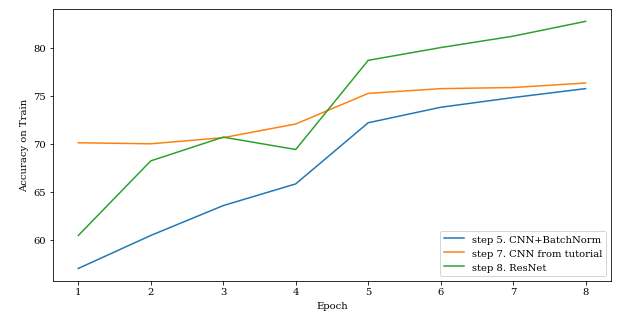
\includegraphics[width=\textwidth, height=7cm]{actrain}	
   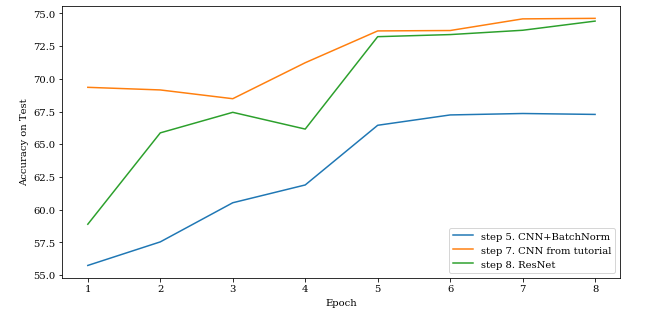
\includegraphics[width=\textwidth, height=7cm]{actest}
   
10) If I had more time I would train more networks and tried an ensamble voting, it always helps me. I hope I will do this, so please check my github and colab notebooks:

       \begin{itemize}
\item https://colab.research.google.com/drive/1cZL-TMTNnrMMesjh17b2\_jF9LDXBZZP4    -- CNN from tutorial
\item https://colab.research.google.com/drive/1A1XGdPsPETG9KJCrLmDFP0ab1O9AT0eR		-- Simple ResNet
\item https://colab.research.google.com/drive/19V32nqQhcxA2YlOwVGeJvjoFcXGiSV82       -- CNN+BatchNorm + model comparison plots
\item https://github.com/Anastasiia-Khab/homeworks-ucu/tree/master/ComputerVision/CV5    --github
       \end{itemize}

Also, all the accuracy in this report are given only after 8 epoch. If to train more epoch models become much more accurate.

\end{document}
